\newpage
\section{Tvorba workflow}
K celkovému workflow se přistupuje jako k orientovanému grafu. V tomto smyslu je graf objekt třídy \textbf{Graph} a vytvoří se při spuštění Workflow Builderu. Vrcholy představují moduly, které jsou třídy Module, a hrany představují spojení, která jsou třídy \textbf{Connection}. Do grafu se postupně přidávají moduly podle toho, jak uživatel pomocí myši přetahuje moduly z Processing Manageru. Objekt třídy Module se vytvoří na základě instance přetaženého modulu (název, popis, tagy a parametry). Modul z Workflow Builderu obsahuje parametry třídy \textbf{Port}. Instance třídy Port se také vytváří automaticky a přiřazují se danému modulu. Grafická reprezentace Module je \textbf{QGraphicsModuleItem}, který také podle \textbf{Port}ů v Module vytvoří \textbf{QGraphicsPortItem}y. Při spojování portů mezi sebou se kontroluje, zdali koresponduje typ parametru (RasterLayerParameter, NumericPrameter, ...), spojuje-li se vstupní parametr s výstupním, zdali nejsou oba parametry parametry stejného modulu a zdali není vstupní parametr prázdný (to znamená, že není spojený s jiným parametrem). Typ a název parametru můžeme zjistit posunutím myši nad parametr (čtvereček - povinný parametr, kolečko - volitelný parametr). Pakliže jsou splněny všechny podmínky, vytvoří se spojení třídy Connection a jeho grafická reprezentace \textbf{QGraphicsConnectionItem}. Connection se poté přidá do Graphu. QGraphicsConnectionItem se přidá do scény (\textbf{DiagramScene}, která je reimplementací třídy QGraphicsScene z Qt). Pro tvorbu spojení stačí kliknout na požadovaný vstup/výstup a táhnout myší na druhý parametr \figurename \ref{wf:crCon}.

\begin{figure}[h]
	\centering
	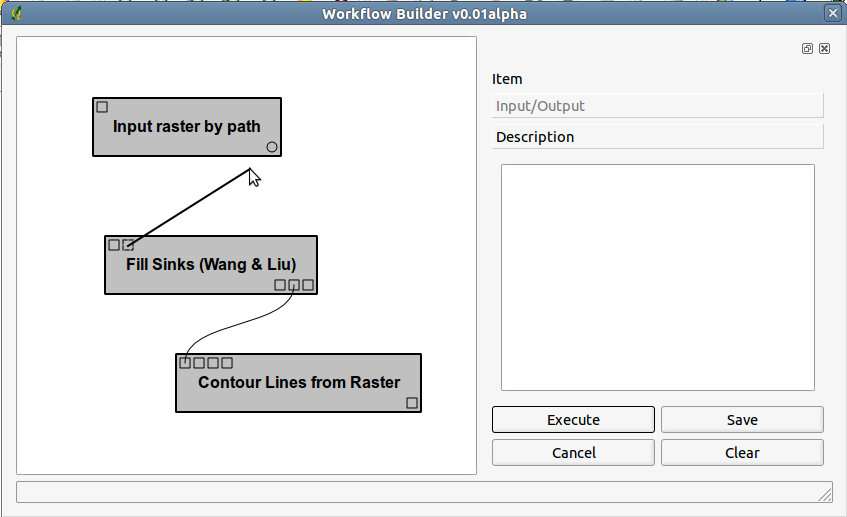
\includegraphics[scale=0.5]{pictures/wf/wf_crCon}
	\caption{Workflow Builder - tvorba spojení}
  	\label{wf:crCon}
\end{figure}

Zrušit modul či spojení můžeme tím, že si jej myší označíme a stiskneme klávesu \textit{Delete}. K mazání prvků se může také použít tlačítko $Clear$ v pravé spodní části dialogového okna, které smaže všechny prvky ve scéně včetně modulů a spojení.

V Graphu máme tedy uloženy moduly a spojení mezi nimi (Module a Connetion). Jsou uloženy jako slovníky, kde klíč je identifikační číslo modulu, resp. spojení a hodnota je instance třídy Module, resp. Connection. Ty se během tvorby workflow mění podle toho, jak uživatel přidává a odebírá moduly, spojuje je a ruší spojení.


%%%%%%
%%% postranni panel
%%%%%%
Po kliknutí na konkrétní modul se zobrazí jeho parametry v pravém postranním panelu. Ty jsou děleny na povinné a volitelné. Toto dělení, podobně jako označení výstupního parametru symbolem "$\rangle$ " před jeho název, bylo převzato z klasického dialogu pro spuštění modulu v QGIS Processing Frameworku. \\

\begin{figure}[h]
	\centering
	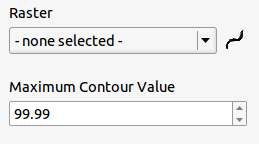
\includegraphics[scale=0.9]{pictures/wf/wf_inPar}
	\caption{Workflow Builder - vstupní parametr}
  	\label{wf:inPar}
\end{figure}

Na \figurename \ref{wf:inPar} je vidět, že widget pro nastavení vstupního parametru se skládá z jeho názvu parametru (QLabel), dále z widgetu, který se generuje na základě jeho typu (podobně jako u QGIS Processing Frameworku) a pakliže je parametr spojen s jiným, objeví se vpravo ikona signalizující spojení. \\

\begin{figure}[h]
	\centering
	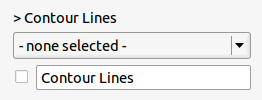
\includegraphics[scale=1.0]{pictures/wf/wf_outPar}
	\caption{Workflow Builder - výstupní parametr}
  	\label{wf:outPar}
\end{figure}

Widget pro nastavení výstupního parametru obsahuje řádek navíc se zaškrtávacím polem (QCheckBox) a textovým polem pro zadání názvu výstupní vrstvy (QLineEdit). Řádek slouží k načtení výstupní vrstvy  do QGIS pod uživatelem zadaným názvem, pakliže zaškrtne zaškrtávací pole. Toto mělo být pouze provizorní řešení. Workflow Builder byl testován s SAGA Pluginem a ten je v současné době napsán tak, že nerespektuje zadaný výstupní parametr a jedná-li se o vrstvu (rastrovou nebo vektorovou), vytvoří novou a tu vždy načte pod náhodně vygenerovaným názvem do QGIS.

Dialogové okno Workflow Builderu spouští a ukládá workflow přes instanci třídy \textbf{Graph}. 